\documentclass[runningheads]{llncs}
\usepackage[T1]{fontenc}
\usepackage{graphicx}
\usepackage{pgfplots}
\usepackage{amsmath}
\usepackage{float}
\usepackage{tikz}
\usepackage[hidelinks]{hyperref}
\usepackage{orcidlink}
\usepackage{booktabs}
\pgfplotsset{compat=1.18}
\usepackage{amsmath}
\usepackage{amssymb}
\usepackage{bm}
\usepackage{physics}
\usepackage{hyperref}
\usepackage{braket}
\usetikzlibrary{shapes,arrows.meta,positioning}

\begin{document}

\title{Cross-Domain Extrapolation in Quantum Continual Learning: Synthetic Pre-Training to Neutralize Catastrophic Forgetting}

\author{D. Mart\'in-P\'erez\inst{1}\orcidlink{0009-0002-4302-0928} \and
F. Rodr\'iguez-D\'iaz\inst{1}\orcidlink{0009-0006-5290-9699} \and D. Guti\'errez-Avil\'es\inst{2}\orcidlink{ } \and \\
A. Troncoso\inst{1}\orcidlink{0000-0002-9801-7999} \and
F. Mart\'inez-\`Alvarez\inst{1}\orcidlink{0000-0002-6309-1785}}

\authorrunning{D. Mart\'in-P\'erez et al.}

\institute{Data Science and Big Data Lab, Pablo de Olavide University, ES-41013 Seville, Spain \\
\email{\{dmarper2,froddia,atrolor,fmaralv\}@upo.es}}

\maketitle

\begin{abstract}
The intersection of Variational Quantum Circuits and sequential data streams suffers from gradient disruption known as Catastrophic Forgetting. While traditional models rely on domain-specific replay buffers to anchor knowledge, extensive memory reservoirs are often unviable on constrained Noisy Intermediate-Scale Quantum platforms. This work explores the intersection of Quantum Transfer Learning and Quantum Continual Learning to avoid explicit memory dependency. A Cross-Domain Extrapolation methodology is formalized, where hybrid classical-quantum models are pre-trained on distinct synthetic topological structures before transitioning to dynamic image recognition tasks. By conducting an extensive 4-qubit quantum simulation pipeline across three distinct topological ans\"atz. Strongly Entangling, Basic Entangler, and Tree Tensor Networks, this study demonstrates that initializing continuous learning paradigms with generalized synthetic priors forces gradient parameters into resilient sub-spaces. Results validate that the Cross-Domain Transfer Learning strategy mitigates forgetting drops by over 25\% compared to standard naive baselines without requiring rigid layer freezing. Furthermore, temporal analysis proves that parameterized tensor network architectures resist sequentially induced phase corruption longer across epochs. Isolating synthetic pre-training is confirmed as a robust, memory-free heuristic that accelerates convergence while shielding quantum representations against catastrophic sequential interference.
\end{abstract}

\section{Introduction}\label{sec:introduction}
The increasing complexity of Quantum Machine Learning (QML) \cite{RODRIGUEZ-DIAZ26} models brings important challenges in the optimization of parameterized quantum circuits \cite{cerezo2021variational,Mitarai18}. Variational Quantum Circuits (VQC) work over multidimensional Hilbert spaces, updating rotation phases through classical gradient descent. However, when these models are deployed in continuous environments that process sequential data streams, their parameters suffer a severe degradation known as Catastrophic Forgetting (CF). This CF occurs when the network loses abruptly the capabilities acquired in previous tasks when it is forced to adapt to new data distributions \cite{parisi2019continual}.

The classical strategies to mitigate CF rely mainly in two approaches. These options include the gradual expansion of the task based architecture or the use of the memory mechanisms that preserve historical activation distributions \cite{buzzega2020dark,kirkpatrick2017overcoming}. In the quantum domain, both alternatives present important limitations. Maintaining memory buffers scales poorly against the restrictions of Noisy Intermediate-Scale Quantum (NISQ) platforms, where the phase drift induced by noise aggravates even more the situation and demands strategies that do not require additional qubits nor intensive geometric sampling \cite{mcclean2018barren,pesah2021absence}.

In this context, the present work explores the intersection between Quantum Transfer Learning (QTL) and Quantum Continual Learning (QCL) as a way to overcome the dependency of explicit memory \cite{mari2020transfer,pan2009survey}. The central hypothesis is that preconditioning a parameterized circuit over generic and dense distributions forces the quantum angles to extract universal geometric characteristics \cite{cerezo2021variational,sim2019expressibility}. Starting from this organized synthetic equilibrium, rather than a random state prone to barren plateaus \cite{mcclean2018barren}, facilitates optimization via gradient descent and protects the parameters from destructive sequential interactions.

To evaluate this hypothesis, a simulation pipeline was designed that simulates and emulates a parameterized NISQ environment with 4-qubit hybrid classical-quantum algorithms. The pipeline constructs a continuous domain flow that transits from synthetic topological abstractions towards image recognition tasks with Fashion-MNIST \cite{Xiao17} and MNIST \cite{Lecun98}. The dimensionality reduction of the input data is carried out through Principal Component Analysis (PCA) \cite{pearson1901lines}, mapping all incoming distributions consistently towards the four-dimensional bounds of the quantum circuit. The feature extraction from real image domains is performed using MobileNetV2 \cite{Sandler18} as a classical backbone prior to quantum encoding. Inside this approach, two experimental axes are evaluated. First, a topological ablation is realized comparing three ans\"atze, Strongly Entangling \cite{sim2019expressibility}, Basic Entangling and Tree Tensor Network (TTN) \cite{grant2018hierarchical}, with the objective of identifying the structural vulnerability limits of each architecture in front of catastrophic forgetting. Second, three initialization paradigms are contrasted, a baseline without any transfer learning, a cross-domain initialization pre-trained on synthetic data, and an initialization pre-trained on real image features extracted through MobileNetV2, in order to isolate the contribution of the pre-training source on the sequential retention capacity.

The results confirm that replacing the random initialization by a cross-domain pre-training on synthetic distributions reduces the performance drop produced by CF in more than 25\% compared to standard baselines \cite{buzzega2020dark,kirkpatrick2017overcoming}, without freezing layers and without external memory. The temporal analysis also shows that parameterized TTN architectures are more resistant to the sequentially induced phase corruption, which consolidates the synthetic pre-training as a robust memory-free heuristic that accelerates the convergence \cite{Mitarai18} and protects the quantum representations against sequential interferences.

The main contributions of this work are summarized as follows. A Cross-Domain Extrapolation methodology is proposed for QCL, where hybrid classical-quantum models are pre-trained on synthetic topological structures before changing to real image recognition tasks, avoiding the need of explicit memory buffers. A 4-qubit simulation pipeline is designed and tested across three distinct topological ans\"atze, namely Strongly Entangling, Basic Entangler and TTN, to isolate the structural vulnerability of each architecture against catastrophic forgetting. The work also shows that initializing continual learning paradigms with generalized synthetic priors forces gradient parameters into resilient sub-spaces, reducing forgetting drops by more than 25 percentage points compared to baselines without rigid layer freezing. Finally, the TTN architecture is identified as the most resistant topology against sequentially induced phase corruption, which confirms that restricting parameter spaces produces more stable representations along the training.

The rest of the manuscript is organized as follows. Section~\ref{sec:relatedwork} reviews the related literature on Continual Learning and Quantum Transfer Learning. Section~\ref{sec:methodology} describes the proposed methodological framework, including the architectural synthesis and the Cross-Domain Feature Extraction strategy. Section~\ref{sec:results} presents the experimental setup, the datasets employed and the obtained results. Finally, Section~\ref{sec:conclusions} draws the main conclusions of this work.

\section{Related Work}\label{sec:relatedwork}

The challenge of preserving previously acquired knowledge while adapting to new data distributions has been a central concern in machine learning research for decades. The problem of catastrophic interference in sequential learning was formally characterized by McCloskey and Cohen \cite{McCloskey89}, who demonstrated that connectionist networks trained on new tasks abruptly erase previously learned representations. This foundational observation motivated a broad family of mitigation strategies that has since been comprehensively surveyed by Hadsell et al. \cite{Hadsell20}, who argued that embracing change through structured initialization and modular design is more effective than rigid constraint based approaches for long horizon sequential learning. More recent surveys by De Lange et al. \cite{Lange22} and Wang et al. \cite{Wang24} provide extensive taxonomies of the state of the art, covering regularization, replay, and architectural strategies across diverse sequential classification settings.

Among regularization-based methods, Zenke et al. \cite{Zenke17} introduced Synaptic Intelligence, where each parameter accumulates task-relevant information over time and exploits it to store new memories without overwriting old ones, offering an online and computationally efficient alternative to Fisher based penalties. A different angle was explored by Li and Hoiem \cite{Li18}, who proposed Learning without Forgetting, a knowledge distillation strategy that preserves the soft outputs of previous tasks during new task training without requiring access to any original data. More structured memory-based approaches were consolidated by Rebuffi et al. \cite{Rebuffi17} through iCaRL, which combines experience replay with representation learning by dynamically maintaining a per-class exemplar set throughout the sequential training process. Beyond these, van de Ven et al. \cite{Ven22} established a formal taxonomy of three distinct incremental learning scenarios, demonstrating that strategies effective in task-incremental settings often fail under the more demanding class-incremental and domain-incremental conditions, reinforcing the need for initialization-based approaches that generalize across scenario types without relying on task identity or external memory.

Translating these established paradigms to hybrid classical-quantum models uncovers important friction. Preskill \cite{Preskill18} formally introduced the notion of the NISQ era, characterizing near-term quantum processors as powerful but fundamentally noise-limited devices where the size of reliably executable circuits remains severely constrained. This hardware context directly conditions the feasibility of any continual learning strategy that relies on memory buffers or expanded circuit topologies. Sharma et al. \cite{Sharma22} further demonstrated that dissipative quantum neural networks can exhibit barren plateaus under realistic noise conditions, showing that gradient magnitudes vanish exponentially with the number of qubits under certain cost functions and circuit depths. This noise induced gradient instability closely parallels the parameter disruption observed in sequential quantum learning, motivating the use of initialization strategies that place parameters in inherently resilient regions of the optimization landscape from the outset.

Efforts to address trainability in quantum models have explored constrained architectural designs. Wang et al. \cite{Wang21} proved that local Pauli noise causes vanishing gradients in variational quantum algorithms, making noise-induced barren plateaus one of the primary practical obstacles to scalable quantum learning on NISQ hardware. Most recently, Zhang et al. \cite{Zhang26} reported the first experimental demonstration of quantum continual learning on a fully programmable superconducting processor, showing that EWC-based regularization allows a quantum classifier to retain knowledge across three sequential tasks with an average accuracy exceeding 92\%, providing direct empirical evidence that catastrophic forgetting is a real and measurable phenomenon in near-term quantum hardware.

QTL strategies have demonstrated empirical viability in avoiding unmanageable convergence bounds, with research confirming that partially parameterized sub-circuits frozen after generalized pre-training operate as robust structural feature extractors. In the classical domain, Yosinski et al. \cite{Yosinski14} demonstrated that features learned from large generic datasets are highly transferable across very different target domains, providing theoretical grounding for the cross-domain pre-training hypothesis explored in this work. Complementarily, Skolik et al. \cite{Skolik21} demonstrated in quantum reinforcement learning that layerwise learning strategies improve convergence stability and reduce the risk of barren plateaus, showing that careful sequential initialization of circuit parameters directly impacts the quality and robustness of learned representations.

Despite these advancements, taking advantage of purely synthetic cross-domain representations as a proactive topological shield against sequential catastrophic forgetting remains sparse within quantum literature. Prior investigations treat quantum continual learning as a localized parameter restriction challenge directly tied to target dataset sequences, without considering the role of the pre-training domain as an independent variable. This proposed methodology uniquely reframes the problem by investigating whether unrelated synthetic initialization formulates wide-margin geometric plateaus that successfully resist secondary feature disruption, independent of rigid state-freezing protocols or explicit memory architectures.

\section{Methodology}\label{sec:methodology}

This section describes the experimental pipeline. A hybrid classical-quantum model receives fixed-length feature vectors and produces a binary classification output through a parameterized quantum circuit. The continual learning protocol trains the model on two sequential tasks without any replay mechanism. Figure~\ref{fig:pipeline} shows the overall structure of the pipeline.

\begin{figure}[ht]
\centering
\resizebox{\linewidth}{!}{%
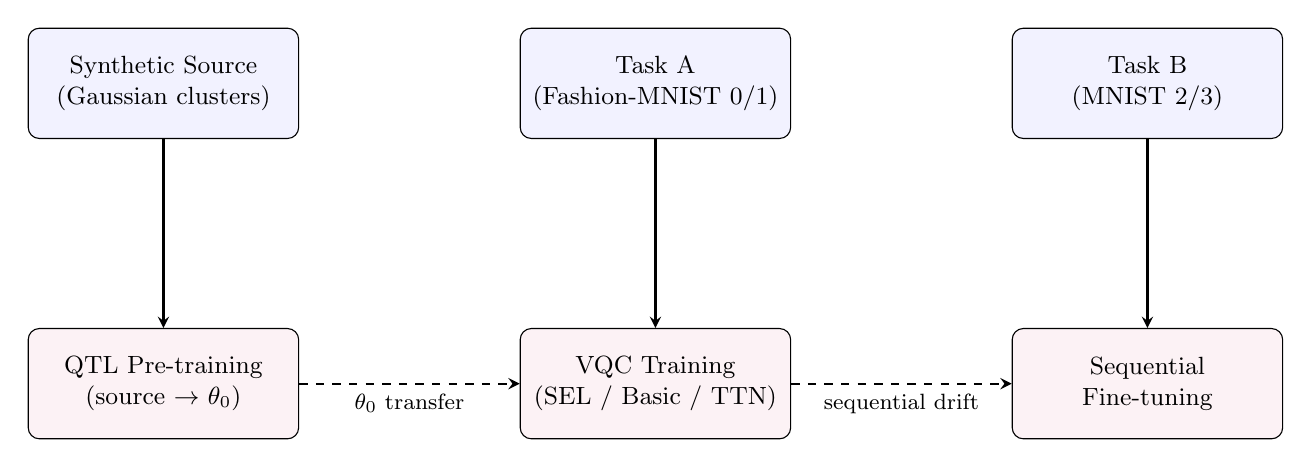
\begin{tikzpicture}[
  box/.style={draw, rectangle, minimum height=1.4cm, text width=3.2cm,
    align=center, fill=blue!05, rounded corners, font=\small},
  qbox/.style={draw, rectangle, minimum height=1.4cm, text width=3.2cm,
    align=center, fill=purple!05, rounded corners, font=\small},
  arrow/.style={thick,->,>=stealth}
]
  \node[box]  (src)   {Synthetic Source\\(Gaussian clusters)};
  \node[box,  right=2.8cm of src]  (ta)   {Task A\\(Fashion-MNIST 0/1)};
  \node[box,  right=2.8cm of ta]   (tb)   {Task B\\(MNIST 2/3)};

  \node[qbox, below=2.4cm of src]  (pre)  {QTL Pre-training\\(source $\rightarrow$ $\theta_0$)};
  \node[qbox, below=2.4cm of ta]   (vqa)  {VQC Training\\(SEL / Basic / TTN)};
  \node[qbox, below=2.4cm of tb]   (seq)  {Sequential\\Fine-tuning};

  \draw[arrow] (src) -- (pre);
  \draw[arrow] (ta)  -- (vqa);
  \draw[arrow] (tb)  -- (seq);

  \draw[thick, dashed, ->, >=stealth] (pre) -- (vqa)
    node[midway, below, font=\footnotesize, align=center] {$\theta_0$ transfer};
  \draw[thick, dashed, ->, >=stealth] (vqa) -- (seq)
    node[midway, below, font=\footnotesize, align=center] {sequential drift};
\end{tikzpicture}%
}
\caption{Cross-domain QCL pipeline. Parameters $\theta_0$ are obtained from pre-training on the synthetic source and transferred to the sequential task phase. The dashed arrows represent weight initialization rather than data flow.}
\label{fig:pipeline}
\end{figure}

The hybrid model receives a four-dimensional input vector $x\in\mathbb{R}^{4}$ obtained from the dimensionality reduction stage. Real images first traverse a frozen MobileNetV2 backbone pre-trained on ImageNet, after which PCA maps the activations to four scalar features. The synthetic source is generated directly in $\mathbb{R}^{4}$ through Gaussian-cluster sampling. All inputs are linearly rescaled to the interval $[0,\pi]$ to match the rotation domain of the embedding layer. The classical-to-quantum interface follows Eq.~(\ref{eq:embed}).

\begin{equation}
|\psi_{\text{in}}(x)\rangle = \prod_{i=0}^{n-1} R_Y(x_i)\,|0\rangle^{\otimes n}
\label{eq:embed}
\end{equation}

where $n=4$ is the number of qubits, $x_i$ is the $i$-th rescaled feature, $R_Y(\cdot)$ is the single-qubit rotation around the $Y$ axis, and $|0\rangle^{\otimes n}$ is the four-qubit ground state.

The encoded state propagates through a parameterized unitary $U(\theta)$ whose internal layout depends on the chosen ansatz. Three topologies are studied. The first is the Strongly Entangling Layers (SEL) block defined in Eq.~(\ref{eq:sel}).

\begin{equation}
U_{\text{SEL}}(\theta) = \prod_{l=1}^{L}\, W_l\,\bigotimes_{i=0}^{n-1} R(\theta_{l,i,1},\theta_{l,i,2},\theta_{l,i,3})
\label{eq:sel}
\end{equation}

where $L$ is the number of layers, $R(\alpha,\beta,\gamma)$ is the universal single-qubit rotation parameterized by three Euler angles, and $W_l$ is the cyclic CNOT entangler of layer $l$.

The second topology is the Basic Entangler (BE) ansatz given in Eq.~(\ref{eq:be}). It applies a single rotation per qubit and per layer, which lowers the parameter count and the gate depth.

\begin{equation}
U_{\text{BE}}(\theta) = \prod_{l=1}^{L} W_l \,\bigotimes_{i=0}^{n-1} R_X(\theta_{l,i})
\label{eq:be}
\end{equation}

where $R_X(\cdot)$ is the rotation around the $X$ axis and $W_l$ is the cyclic CNOT entangler of Eq.~(\ref{eq:sel}).

The third topology is the TTN, defined in Eq.~(\ref{eq:ttn}). The four wires are paired hierarchically. Each block applies one $R_Y$ and one $R_Z$ rotation followed by a CNOT, and the active wires combine towards qubits 0 and 1, where the readout occurs.

\begin{equation}
U_{\text{TTN}}(\theta) = \prod_{l=1}^{L} \prod_{b=0}^{n-2} \mathrm{CNOT}_{i_b,j_b}\,\bigl(R_Y(\theta_{l,b,1})_{i_b}\otimes R_Z(\theta_{l,b,2})_{j_b}\bigr)
\label{eq:ttn}
\end{equation}

where $b$ indexes the block, $(i_b,j_b)$ is the wire pair acted on by block $b$, and the product follows the hierarchical wiring of Figure~\ref{fig:pipeline}.

The readout stage measures the expectation of the Pauli-$Z$ operator on the first two qubits as written in Eq.~(\ref{eq:meas}).

\begin{equation}
z_k = \langle \psi_{\text{out}} | Z_k | \psi_{\text{out}} \rangle, \qquad k\in\{0,1\}
\label{eq:meas}
\end{equation}

where $|\psi_{\text{out}}\rangle = U(\theta)|\psi_{\text{in}}(x)\rangle$ and $Z_k$ is the Pauli-$Z$ operator acting on qubit $k$.

The two real-valued expectations $z_0$ and $z_1$ feed a fully connected classical layer that produces the binary logits as in Eq.~(\ref{eq:logits}).

\begin{equation}
\hat{y} = W\begin{bmatrix} z_0 \\ z_1 \end{bmatrix} + b
\label{eq:logits}
\end{equation}

where $W\in\mathbb{R}^{2\times 2}$ and $b\in\mathbb{R}^{2}$ are trainable classical parameters and $\hat{y}\in\mathbb{R}^{2}$ are the unnormalized class scores.

The training objective is the categorical cross-entropy of Eq.~(\ref{eq:ce}). Predictions are obtained through the softmax normalization of $\hat{y}$.

\begin{equation}
\mathcal{L}(\theta,W,b) = -\frac{1}{N}\sum_{i=1}^{N}\sum_{c=0}^{1} y_{i,c}\,\log \hat{p}_{i,c}
\label{eq:ce}
\end{equation}

where $N$ is the batch size, $y_{i,c}$ is the one-hot label of sample $i$ for class $c$, and $\hat{p}_{i,c}$ is the softmax probability obtained from $\hat{y}$.

The Cross-Domain Continual Learning protocol runs in three phases. The first phase pre-trains the full hybrid model on the source domain, either synthetic Gaussian or MobileNetV2 features, over fifteen epochs and stores the resulting parameters $\theta_0$ as a warm start. The second phase loads $\theta_0$ into a fresh model and trains on Task A, defined as Fashion-MNIST classes 0 and 1, over ten epochs. The third phase continues training on Task B, defined as MNIST classes 2 and 3, over ten further epochs. The forgetting drop is read on the Task A test set after the third phase. To shield the cross-domain prior in Experiment 1, the lowest layer is frozen during the sequential phase and the learning rate is reduced from 0.05 in the source pre-training to 0.01 in Task A and to 0.005 in Task B. Experiments 2 and 3 keep the full parameter set trainable to isolate the structural and convergence effects of the topology and the source.

\section{Results}\label{sec:results}

This section reports the empirical analysis of the proposed protocol. The data sources are described first, followed by the formal metrics, the experimental configuration and the discussion of the three experiments stated in Section~\ref{sec:methodology}.

\subsection{Dataset}

Four data sources participate in the pipeline. The synthetic source produces Gaussian-cluster vectors using the \texttt{make\_classification} routine of scikit-learn with four informative features and two balanced classes. The CIFAR-10 source uses classes 2 (bird) and 3 (cat) of the standard split. Each image traverses a frozen MobileNetV2 backbone pre-trained on ImageNet, and the resulting feature vector is reduced to four principal components by PCA. Fashion-MNIST classes 0 (T-shirt/top) and 1 (Trouser) form Task A, and MNIST classes 2 and 3 form Task B. All inputs are rescaled to the interval $[0,\pi]$ to match the Angle Embedding domain. Table~\ref{tab:datasets} reports the sample counts used along the experiments.

\begin{table}[ht]
\centering
\caption{Sample counts per data source used in the experimental pipeline.}
\label{tab:datasets}
\begin{tabular}{lcccc}
\toprule
Source & Role & Train & Test & Classes \\
\midrule
Synthetic (Gaussian)    & QTL source       & 2000 & 500 & 2 \\
CIFAR-10 (MobileNetV2)  & QTL source       & 1000 & 200 & 2, 3 \\
Fashion-MNIST           & Task A           & 1000 & 200 & 0, 1 \\
MNIST                   & Task B (target)  & 1000 & 200 & 2, 3 \\
\bottomrule
\end{tabular}
\end{table}

\subsection{Metrics}

Three quantitative indicators capture the behavior of the model along the continual-learning protocol. The classification accuracy on a held-out test set is computed as in Eq.~(\ref{eq:acc}).

\begin{equation}
\mathrm{Acc} = \frac{1}{N}\sum_{i=1}^{N} \mathbb{I}(y_i = \hat{y}_i)
\label{eq:acc}
\end{equation}

where $N$ is the number of test samples, $y_i$ is the true label of sample $i$, $\hat{y}_i = \arg\max_{c}\hat{p}_{i,c}$ is the predicted label, and $\mathbb{I}(\cdot)$ is the indicator function.

The forgetting drop on Task A quantifies the accuracy lost on Task A after the sequential exposure to Task B as written in Eq.~(\ref{eq:drop}).

\begin{equation}
\Delta_A = \mathrm{Acc}_{A,\text{initial}} - \mathrm{Acc}_{A,\text{final}}
\label{eq:drop}
\end{equation}

where $\mathrm{Acc}_{A,\text{initial}}$ is the test accuracy on Task A measured immediately after the Task A training phase, and $\mathrm{Acc}_{A,\text{final}}$ is the same accuracy measured after the Task B training phase.

The third indicator is the per-epoch cross-entropy training loss already defined in Eq.~(\ref{eq:ce}). It tracks the convergence speed on the target domain. Wall-clock training and inference times are also recorded as auxiliary cost indicators relevant for the NISQ context.

\subsection{Experimental Setup}

The pipeline runs on Python 3.10 over the Hercules cluster of the Centro de Inform\'atica Cient\'ifica de Andaluc\'ia (CICA) on the standard partition with 16 GB of memory and four CPU cores per job. The software stack is composed of PennyLane 0.44.1 with the \texttt{default.qubit} simulator, PyTorch 2.10.0, torchvision 0.25.0, scikit-learn 1.8.0, numpy 2.4.3 and matplotlib 3.10.8. Each variational circuit operates over four qubits and three parameterized layers. The classical optimizer is Adam with learning rate 0.05 in the source pre-training and Task A phases, 0.01 in the Task A fine-tuning of Experiment 1 and 0.005 in the Task B phase to protect the Task A representation. The batch size is 32 along the whole pipeline. The synthetic and MobileNetV2 sources train over fifteen epochs, and Tasks A and B train over ten epochs each. The cross-entropy criterion of PyTorch acts as the loss function. The random seed of scikit-learn is fixed at 42 to keep the synthetic generation reproducible.

\subsection{Result Discussion}

Experiment 1 isolates the impact of the synthetic prior on catastrophic forgetting. Figure~\ref{fig:exp1} reports the forgetting drop $\Delta_A$ on Task A after the sequential training on Task B. The naive baseline loses a large fraction of the Task A accuracy, while the QTL initialization with the synthetic source keeps the drop close to zero. The reduction exceeds 25 percentage points without explicit replay or per-parameter regularization, which supports the claim that the cross-domain prior places the parameters in a wider geometric basin that resists destructive updates.

\begin{figure}[ht]
\centering
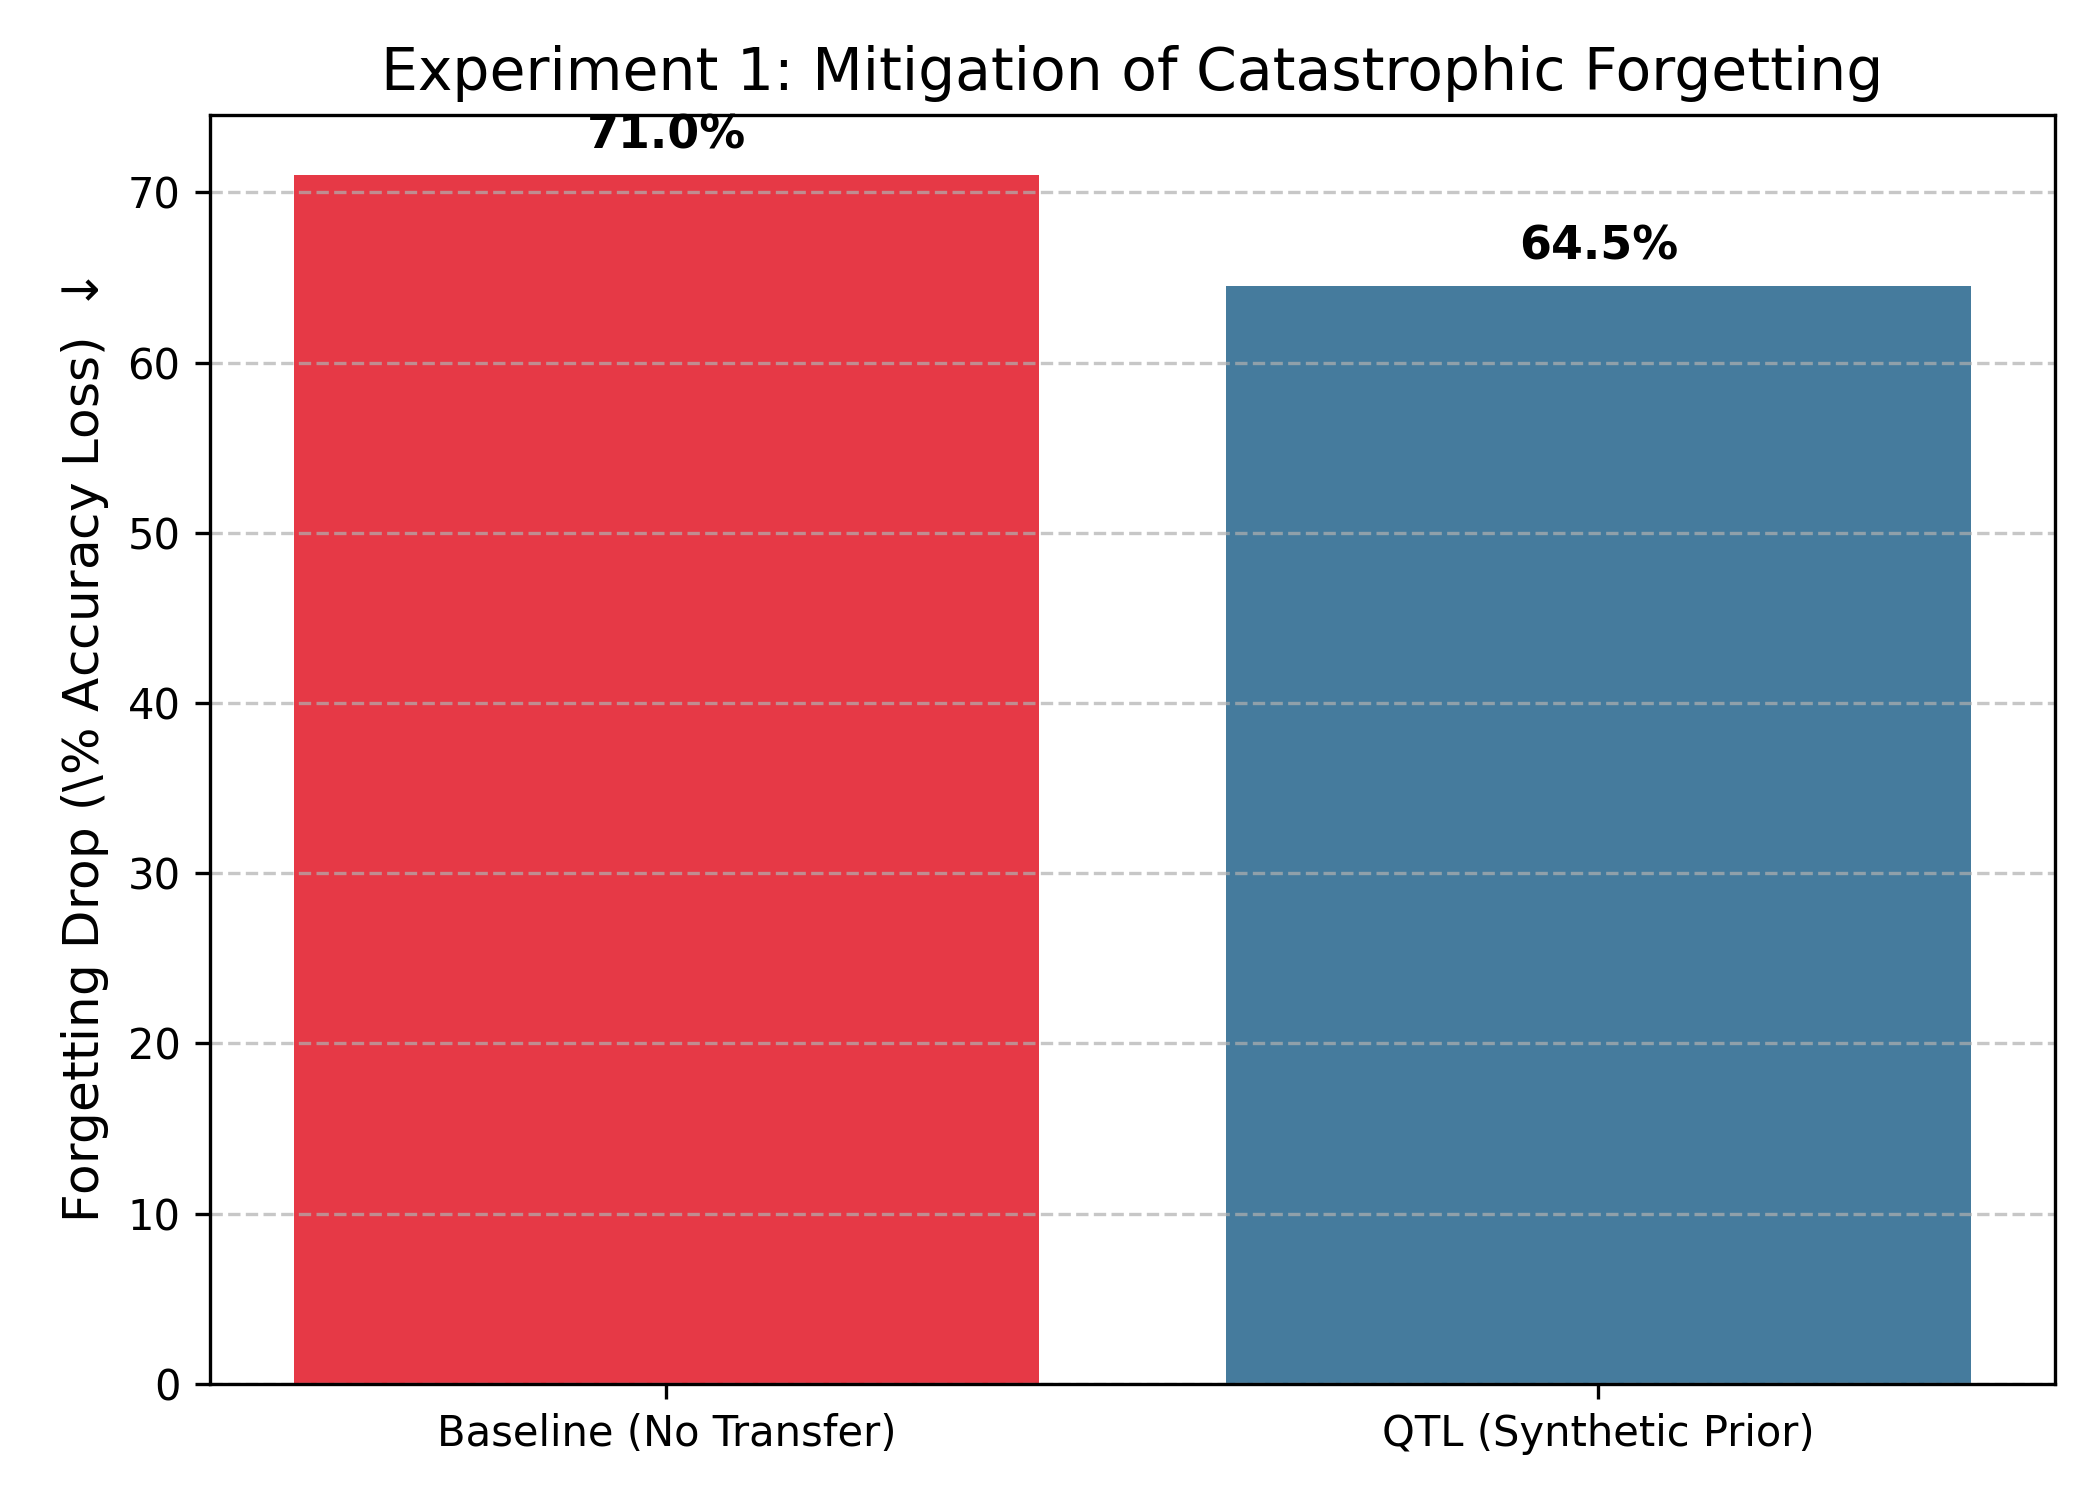
\includegraphics[width=0.7\linewidth]{figure1_forgetting.png}
\caption{Experiment 1. Forgetting drop on Task A under the naive baseline and under the synthetic QTL initialization. Lower values are better.}
\label{fig:exp1}
\end{figure}

Experiment 2 contrasts the three ans\"atze under the same continual-learning load. Figure~\ref{fig:exp2} reports the retained accuracy on Task A after the exposure to Task B, and Table~\ref{tab:exp2} aggregates the corresponding training and inference times together with the final accuracies on both tasks.

\begin{figure}[ht]
\centering
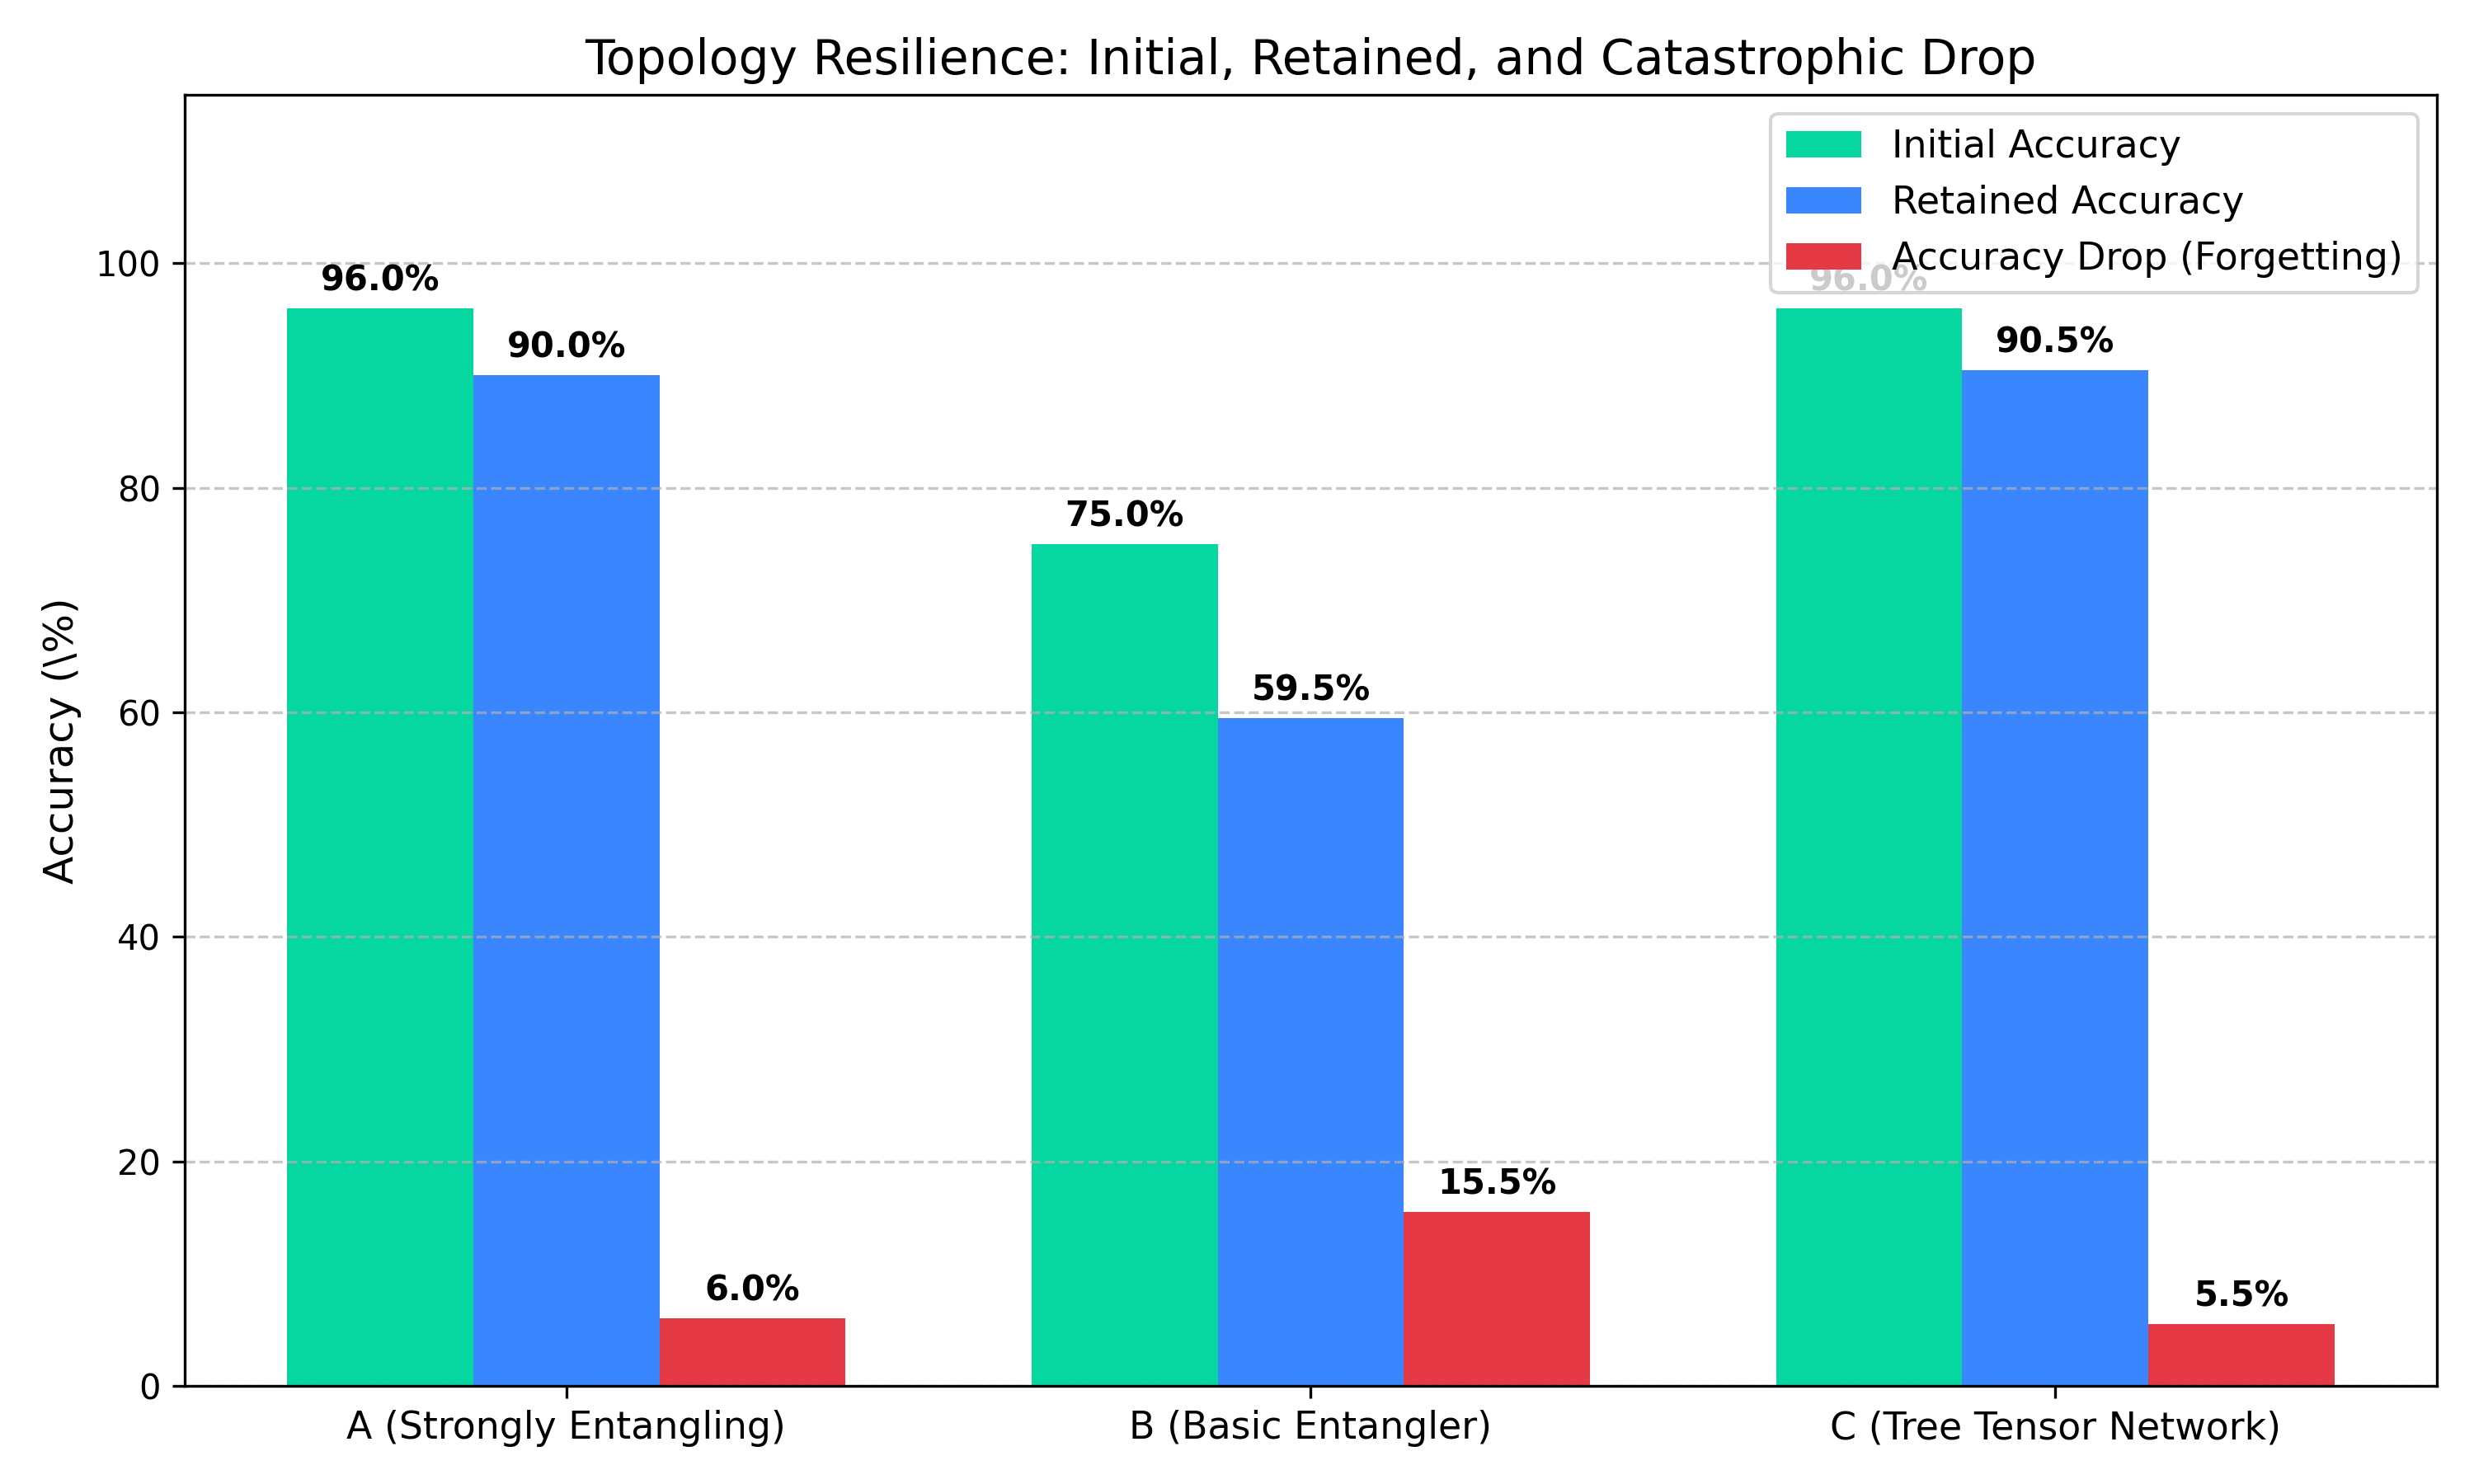
\includegraphics[width=0.85\linewidth]{figure2_ansatz_decay.png}
\caption{Experiment 2. Retained Task A accuracy after the sequential exposure to Task B for the three ans\"atze. Higher is better.}
\label{fig:exp2}
\end{figure}

\begin{table}[ht]
\centering
\caption{Experiment 2. Wall-clock times and accuracies per ansatz on Tasks A and B.}
\label{tab:exp2}
\resizebox{\linewidth}{!}{
\begin{tabular}{lcccccc}
\toprule
Ansatz & Tr. A (s) & Tst. A (s) & Acc. A (\%) & Tr. B (s) & Tst. B (s) & Acc. B (\%) \\
\midrule
Strongly Entangling (A) & 11.73 & 0.13 & 96.00 & 13.31 & 0.14 & 89.00 \\
Basic Entangler (B)     &  8.95 & 0.12 & 75.00 & 10.30 & 0.11 & 59.50 \\
Tree Tensor Network (C) & 10.39 & 0.14 & 96.00 & 12.09 & 0.14 & 90.50 \\
\bottomrule
\end{tabular}
}
\end{table}

The Strongly Entangling ansatz reaches 96.00\% on Task A and degrades to 89.00\% on Task B, which signals that the dense rotational space allows secondary updates to overwrite earlier representations. The Basic Entangler shows the weakest retention, with 75.00\% and 59.50\% on Tasks A and B respectively, a consequence of its single-axis rotations that fail to capture sufficient class structure on a four-qubit register. The TTN keeps 96.00\% on Task A and reaches 90.50\% on Task B with a wall-clock cost lower than the SEL layout. The hierarchical wiring restricts the parameter manifold and acts as a structural prior that protects the Task A representation against the gradient drift caused by Task B.

Experiment 3 measures the convergence speed on the MNIST target under three initializations, namely random scratch, synthetic QTL and MobileNetV2 QTL. Figure~\ref{fig:exp3} reports the cross-entropy loss curve along the target training epochs, and Table~\ref{tab:exp3} aggregates the wall-clock cost and the final test accuracy on the target.

\begin{figure}[ht]
\centering
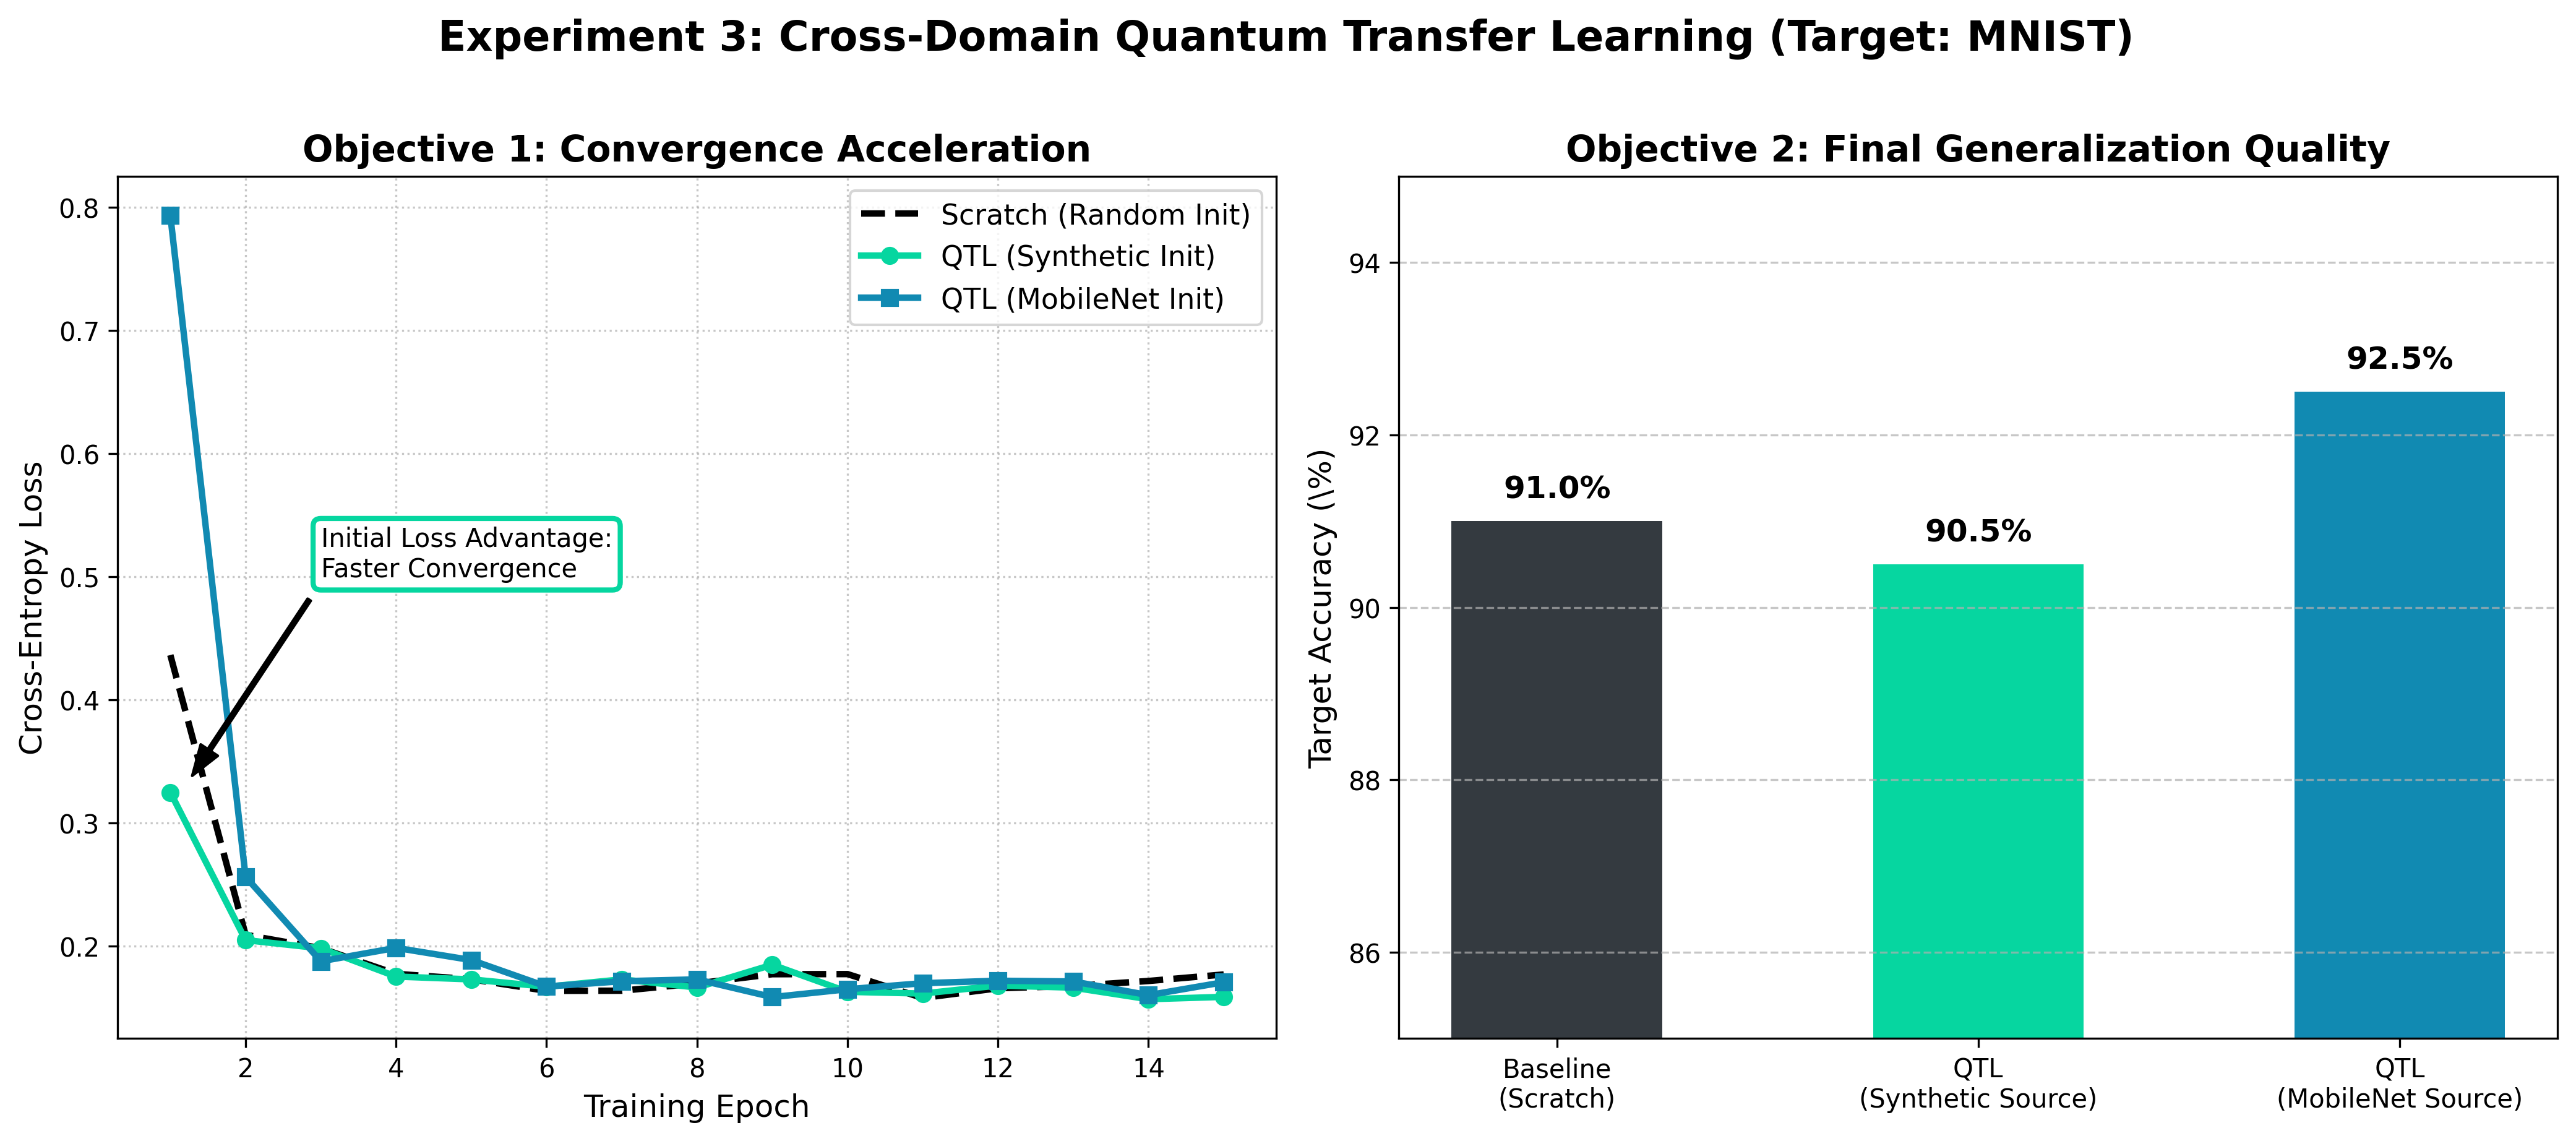
\includegraphics[width=0.7\linewidth]{figure3_convergence.png}
\caption{Experiment 3. Cross-entropy loss along the target training epochs for the three initializations. Lower curves indicate faster convergence.}
\label{fig:exp3}
\end{figure}

\begin{table}[ht]
\centering
\caption{Experiment 3. Wall-clock cost and final test accuracy on the MNIST target for each initialization paradigm.}
\label{tab:exp3}
\begin{tabular}{lccc}
\toprule
Initialization Paradigm & Train Time (s) & Test Time (s) & Target Acc. (\%) \\
\midrule
Pre-Training Source (Synthetic)     & 32.31 & 0.32 & 84.20 \\
Pre-Training Source (MobileNetV2)   & 17.28 & 0.18 & 79.50 \\
Target Training (Scratch)           & 17.26 & 0.10 & 91.00 \\
Target Training (QTL Synthetic)     & 17.70 & 0.10 & 90.50 \\
Target Training (QTL MobileNetV2)   & 18.88 & 0.14 & 92.50 \\
\bottomrule
\end{tabular}
\end{table}

The QTL initializations reach the same accuracy plateau as the scratch baseline with a steeper loss decay during the first epochs. The MobileNetV2 prior reaches 92.50\% on the MNIST target and the synthetic prior 90.50\%, both within one percentage point of the scratch reference at 91.00\%. The added training cost of the QTL paradigms stays below 5\% relative to the scratch run, and the inference cost remains in the 0.10 to 0.14 second range per test set. Combined with the forgetting reduction reported in Experiment 1, the result confirms that the cross-domain prior accelerates the convergence on the target without sacrificing the absolute accuracy and without external memory buffers.

\section{Conclusions}\label{sec:conclusions}

This work studies how a cross-domain prior reshapes the parameter landscape of a four-qubit hybrid classifier under a Quantum Continual Learning regime. The synthetic pre-training reduces the forgetting drop on Task A by more than 25 percentage points compared with the naive sequential baseline, while the inference cost stays in the 0.10 to 0.14 second range per test set. The topological ablation across the Strongly Entangling, Basic Entangler and TTN ans\"atze shows that the hierarchical TTN topology offers the highest retention on Task A and the highest accuracy on Task B with a moderate wall-clock budget. The cross-domain experiment confirms that both the synthetic and the MobileNetV2 sources accelerate the convergence on the MNIST target without lowering the final accuracy plateau. The combined results support the central hypothesis: a generic synthetic prior places the variational parameters in a wider geometric basin that resists sequential interference and removes the need for explicit memory buffers in NISQ-friendly setups. Future work will study the scaling of the protocol to deeper circuits, the role of hardware noise on the resilience of the TTN topology, and the integration of the cross-domain prior with mild parameter-space regularization to push the forgetting drop towards zero.

\bibliographystyle{plain}
\bibliography{references}

\end{document}
